% CAP description for Toolbar Item

Toolbar items are buttons and their menus on a toolbar, such as the one in the \ite{} (\bxfigref{toolbar}). Each of the buttons on the toolbar is a toolbar item. 

\begin{figure}
\begin{center}

\includegraphics{PS/toolbar}
\caption{Toolbar items}
\label{toolbar}
\end{center}
\end{figure}

Often, toolbar items have drop-down menus (\bxfigref{toolbarmenu}).
\begin{figure}
\begin{center}
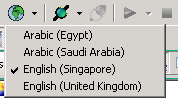
\includegraphics{PS/toolbarmenu}
\caption{Toolbar item menu}
\label{toolbarmenu}
\end{center}
\end{figure}


\textbf{Mapping toolbar items}

In the \gdomm{}, a toolbar item to be mapped looks like this:

\begin{figure}
\begin{center}
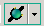
\includegraphics{PS/maptoolbar}
\caption{Mapping toolbar items}
\label{maptoolbar}
\end{center}
\end{figure}
